\documentclass[a4paper,titlepage]{article}
\usepackage[utf8]{inputenc}
\usepackage{fullpage}
\usepackage{indentfirst}
\usepackage[per-mode=symbol]{siunitx}
\usepackage{listings}
\usepackage{graphicx}
\usepackage{color}
\usepackage{amsmath}
\usepackage{array}
\usepackage[hidelinks]{hyperref}
\usepackage[format=plain,font=it]{caption}
\usepackage{subcaption}
\usepackage{standalone}
\usepackage[nottoc]{tocbibind}
\usepackage[noabbrev,capitalize,nameinlink]{cleveref}
\usepackage{listings}
\usepackage{titlesec}
\usepackage{minted}
\usepackage{booktabs}
\usepackage{csvsimple}
\usepackage{siunitx}
\usepackage[super]{nth}
\usepackage[titletoc]{appendix}

% Custom commands
\newcommand\numberthis{\addtocounter{equation}{1}\tag{\theequation}}
\newcommand{\code}[1]{\texttt{#1}}
\newcolumntype{P}[1]{>{\centering\arraybackslash}p{#1}}

\setminted{linenos,breaklines,fontsize=auto}

%\titleformat*{\section}{\normalsize\bfseries}
%\titleformat*{\subsection}{\small\bfseries}
\renewcommand{\thesubsection}{\thesection.\alph{subsection}}
\providecommand*{\listingautorefname}{Listing}
\newcommand*{\Appendixautorefname}{Appendix}
%\crefname{appendix}{Appendix}{Appendices}
%\def\appendixname{Appendix}


%opening
\title{\textbf{ECSE 543 \\ Assignment 2}}
\author{Sean Stappas \\ 260639512}
\date{November \nth{20}, 2017}

\begin{document}
	\sloppy
	\maketitle
	
	\tableofcontents
	
	
	\twocolumn
	
	\section*{Introduction}
	
	The code for this assignment was created in Python 2.7 and can be seen in \autoref{appendix:code}. To perform the required tasks in this assignment, the \mintinline{python}{Matrix} class from Assignment 1 was used, with useful methods such as add, multiply, transpose, etc. This package can be seen in the \mintinline{python}{matrices.py} file shown in \autoref{lst:matrices}. The only packages used that are not built-in are those for creating the plots for this report, i.e., \mintinline{python}{matplotlib} for plotting. The structure of the rest of the code will be discussed as appropriate for each question. Output logs of the program are provided in \autoref{appendix:logs}. The \mintinline{python}{SIMPLE2D} input and output files can be seen in \autoref{appendix:simple2d}.
	
	
	
	\section{Finite Element Triangles}
	
	The source code for the Question 1 program can be seen in the \mintinline{python}{q1.py} file shown in \cref{lst:q1}.
	
	\subsection{Local S-Matrix}
	
	The equation for the $\alpha$ parameter for a general vertex $i$ of a finite element triangle can be seen in \cref{eq:alpha}, where $i+1$ and $i+2$ implicitly wraps around when exceeding 3.
	
	\begin{equation} \label{eq:alpha}
		\begin{split}
			\alpha_i(x, y) = \frac{1}{2A} \big[
			& (x_{i+1}y_{i+2} - x_{i+2}y_{i+1}) \\
			& + (y_{i+1} - y_{i+2})x \\
			& + (x_{i+2} - x_{i+1})y \big]
		\end{split}
	\end{equation}
	
	Using \cref{eq:alpha}, we can solve for the entries of the local $S$ matrix, as shown in \cref{eq:local_s}. This was used in the program to compute every entry for both example triangles.
	
	\begin{equation} \label{eq:local_s}
		\begin{split}
			S_{ij} 
			= &\int\displaylimits_{\Delta_e}\nabla\alpha_i\cdot\nabla\alpha_j dS \\
			= &\frac{1}{4A} \big[ (y_{i+1} - y_{i+2})(y_{j+1} - y_{j+2}) \\
			&+ (x_{i+2} - x_{i+1})(x_{j+2} - x_{j+1})
			\big]
		\end{split}
	\end{equation}
	
	The local $S$-matrix for the first triangle can be seen in \cref{eq:local_s1}.
	
	\begin{equation} \label{eq:local_s1}
		S_1 =
			\begin{bmatrix}
				\input{matrices/S1.txt}
			\end{bmatrix}
	\end{equation}
	
	The local $S$-matrix for the second triangle can be seen in \cref{eq:local_s2}.
	
	\begin{equation} \label{eq:local_s2}
		S_2 =
			\begin{bmatrix}
				\input{matrices/S2.txt}
			\end{bmatrix}
	\end{equation}
	
	\subsection{Global S-Matrix}
	
	The disjoint $S$-matrix is then given by the following:

	\begin{equation*}
		S_{dis} =
			\begin{bmatrix}
				\input{matrices/S_dis.txt}
			\end{bmatrix}
	\end{equation*}
	
	The connectivity matrix $C$ is given by \cref{eq:connectivity}.

	\begin{equation} \label{eq:connectivity}
		C =
			\begin{bmatrix}
				\input{matrices/C.txt}
			\end{bmatrix}
	\end{equation}
	
	The global $S$-matrix is then given by \cref{eq:global_s}.
	
	\begin{equation} \label{eq:global_s}
		S = C^T S_{dis} C^T
	\end{equation}
	
	Using \cref{eq:connectivity,eq:global_s}, we can solve for the global $S$-matrix, giving the value shown in \cref{eq:global_s_solution}, which is computed by the \mintinline{python}{finite_element_triangles.py} script shown in \cref{lst:finite_element_triangles}.
	
	\begin{equation} \label{eq:global_s_solution}
		S =
			\begin{bmatrix}
				\input{matrices/S.txt}
			\end{bmatrix}
	\end{equation}
	
	\section{Finite Element Coaxial Cable}
	
	The source code for the Question 2 program can be seen in the \mintinline{python}{q2.py} file shown in \cref{lst:q2}.
	
	\subsection{Mesh}
	
	The mesh to be used by the \mintinline{python}{SIMPLE2D} program is generated by the \mintinline{python}{finite_element_mesh_generator.py} script shown in \cref{lst:finite_element_mesh_generator}. This input and output files of the \mintinline{python}{SIMPLE2D} program are shown in \cref{lst:mesh,lst:result} of \autoref{appendix:simple2d}.
	
	\subsection{Electrostatic Potential}
	
	Based on the results from the \mintinline{python}{SIMPLE2D} program, the potential at (0.06, 0.04) is \SI{5.5263}{\volt}. This corresponds to node 16 in the mesh arrangement we created.
	
	\subsection{Capacitance}
	
	The finite element functional equation for two conjoint finite element triangles forming a square $i$ can be seen in \cref{eq:functional}.
	
	\begin{equation} \label{eq:functional}
		W_i = \frac{1}{2} U_{con_i}^T S U_{con_i}
	\end{equation}
	where $S$ is given in \cref{eq:global_s_solution} and $U_{con_i}$ is the conjoint potential vector for square $i$, giving the potential at the four corners of the square defining the combination of two finite element triangles. This can be seen in \cref{eq:u}.
	
	\begin{equation} \label{eq:u}
		U_{con} = 
			\begin{bmatrix}
				U_{i_1} \\
				U_{i_2} \\
				U_{i_3} \\
				U_{i_4}
			\end{bmatrix}
	\end{equation}
	
	To find the total energy function $W$ of the mesh, we must add the contributions from each square and multiply by 4, since our mesh is one quarter of the entire coaxial cable. This yields \cref{eq:total_functional}.
	
	\begin{equation} \label{eq:total_functional}
		W = 4 \sum_{i}^{N}{W_i} = 2 \sum_{i}^{N}{U_{con_i}^T S U_{con_i}}
	\end{equation} 
	where $N$ is the number of finite difference squares in the mesh.
	
	Note that $W$ is not equal to the energy. The relation between the energy per unit length $E$ and $W$ is shown in \cref{eq:energy}.
	
	\begin{equation} \label{eq:energy}
		E = \epsilon_0 W
	\end{equation}
	
	We then know that the energy per unit length $E$ is related to the capacitance per unit length $C$ as shown in \cref{eq:energy_capacitor}.
	
	\begin{equation} \label{eq:energy_capacitor}
		E = \frac{1}{2} C V^2
	\end{equation}
	where $V$ is the voltage across the coaxial cable.
	
	Combining \cref{eq:functional,eq:total_functional,eq:energy,eq:energy_capacitor}, we obtain an expression for the capacitance per unit length which can be easily calculated, as shown in \autoref{eq:capacitance}.
	
	\begin{equation} \label{eq:capacitance}
		C = \frac{2E}{V^2} = \frac{4 \epsilon_0}{V^2} \sum_{i}^{N}{U_{con_i}^T S U_{con_i}}
	\end{equation}
	
	The capacitance per unit length is computed as \SI{5.2137E-11}{\farad\per\meter} by the \mintinline{python}{finite_element_capacitance.py} script shown in \cref{lst:finite_element_capacitance} with output shown in \cref{lst:q2_log}.
	
	\section{Conjugate Gradient Coaxial Cable}
	
	The source code for the Question 3 program can be seen in the \mintinline{python}{q3.py} file shown in \cref{lst:q3}.
	
	\subsection{Positive Definite Test}
	
	To form the $A$ matrix, we must consider all the free nodes in the mesh. The potential at the non-boundary free nodes is given by \cref{eq:free_node}.
	
	\begin{equation} \label{eq:free_node}
		-4\phi_{i, j} + \phi_{i + 1, j}  + \phi_{i - 1, j}  + \phi_{i, j + 1}  + \phi_{i, j - 1} = 0
	\end{equation}
	
	The free nodes along a boundary must satisfy the Neumann boundary condition for symmetry. Since our quarter-mesh is the bottom left corner of the overall mesh, these boundary nodes defining planes of symmetry are along the top and the right. The Neumann boundary condition for the top nodes is given by \cref{eq:neumann_top} and that for the right nodes is given by \cref{eq:neumann_right}.

	\begin{equation} \label{eq:neumann_top}
		\phi_{i, j + 1} - \phi_{i, j - 1} = 0
	\end{equation}
	
	\begin{equation} \label{eq:neumann_right}
		\phi_{i + 1, j} - \phi_{i - 1, j} = 0
	\end{equation}
	
	Now, the simplified potential for boundary free nodes can be calculated, as seen in \cref{eq:top_potential,eq:right_potential}.
	
	\begin{equation} \label{eq:top_potential}
		-4\phi_{i, j} + \phi_{i + 1, j}  + \phi_{i - 1, j}  + 2\phi_{i, j - 1} = 0
	\end{equation}
	
	\begin{equation} \label{eq:right_potential}
		-4\phi_{i, j} + 2\phi_{i - 1, j} + \phi_{i, j + 1}  + \phi_{i, j - 1} = 0
	\end{equation}
	
	The non-free nodes are fixed by the potentials of the conductors, i.e., \SI{15}{\volt} and \SI{0}{\volt}.
	
	With \cref{eq:free_node,eq:top_potential,eq:right_potential}, we can form the $A$ matrix from every mesh node. This is done in \mintinline{python}{finite_difference_mesh_generator.py}, as shown in \cref{lst:finite_difference_mesh_generator}. The output $A$ matrix can be seen in \cref{lst:q3_log}.
	
	If the matrix $A$ is not positive definite, one can simply multiply both sides of the $Ax = b$ equation by $A^T$, forming a new equation $A^TAx = A^Tb$. This is equivalent to $A'x = b'$, where $b' = A^Tb$ and $A' = A^TA$. Here, $A'$ is now positive definite.

	In our case, the matrix $A$ is indeed not positive definite, and multiplying by $A^T$ made it positive definite. The before and after positive definite test can be seen in \cref{lst:q3_log}.
	
	\subsection{Matrix Solution}
	
	The matrix equation to be solved can be seen in \cref{eq:fd}, where $A$ is positive-definite matrix generated previously, $\phi_c$ is the unknown potential vector and $b$ contains the initial potential values along the boundaries.
	
	\begin{equation} \label{eq:fd}
		A\phi_c = b
	\end{equation}
	
	The matrix equation is solved first by the Choleski method from Assignment 1 is applied, as found in the \mintinline{python}{choleski.py} shown in \cref{lst:choleski}. Then, the conjugate gradient method defined by \mintinline{python}{conjugate_gradient_solve} of the \mintinline{python}{conjugate_gradient.py} file shown in \cref{lst:conjugate_gradient} was applied. The solved $x$ vector from both methods can be seen in \cref{lst:q3_log}.
	
	\subsection{Residual Norm}
	
	Consider a vector $\textbf{v} = \{v_1, \ldots, v_n\}$. The infinity norm $\|\textbf{v}\|_\infty$ of $\textbf{v}$ is given by the maximum absolute element of $\textbf{v}$, as shown in \cref{eq:infinity_norm}.
	
	\begin{equation} \label{eq:infinity_norm}
		\|\textbf{v}\|_\infty = \max\{|v_1|, \ldots, |v_n|\}
	\end{equation}
	
	Similarly, the 2-norm $\|\textbf{v}\|_2$ of $\textbf{v}$ is given by \cref{eq:2_norm}.
	
	\begin{equation} \label{eq:2_norm}
		\|\textbf{v}\|_2 = \sqrt{\sum_{i = 1}^{n} v_i^2}
	\end{equation}
	
	The infinity norm of the residual vector versus conjugate gradient iterations can be seen in \cref{fig:q3c_infinity}. The 2-norm versus iterations can be seen in \cref{fig:q3c_2}. Both norms converge to 0 after $n = 19$ iterations, as expected.
	
	\begin{figure}[!htb]
		\centering
		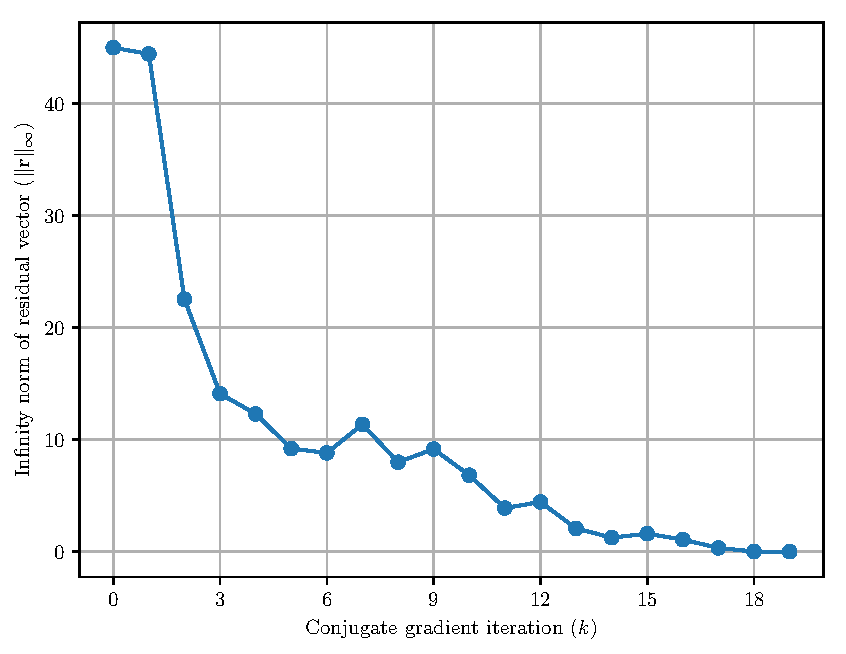
\includegraphics[width=\columnwidth]{plots/q3c_infinity.pdf}
		\caption
		{Value of the infinity norm $\|\textbf{r}\|_\infty$ of the residual vector versus iterations of the conjugate gradient algorithm.}
		\label{fig:q3c_infinity}
	\end{figure}
	
	\begin{figure}[!htb]
		\centering
		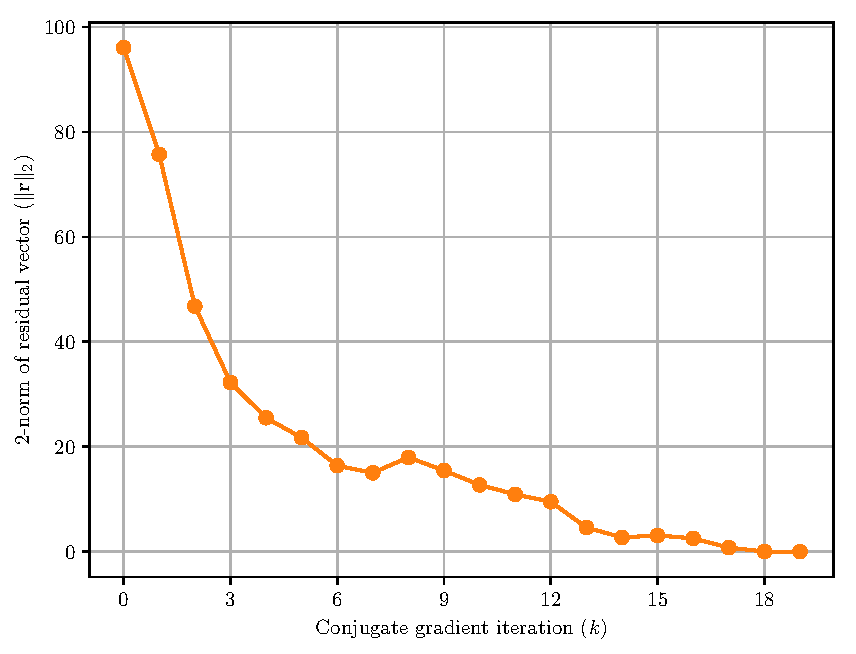
\includegraphics[width=\columnwidth]{plots/q3c_2.pdf}
		\caption
		{Value of the 2-norm $\|\textbf{r}\|_2$ of the residual vector versus iterations of the conjugate gradient algorithm.}
		\label{fig:q3c_2}
	\end{figure}

	\subsection{Potential Comparison}
	
	A comparison of the potential at (0.06, 0.04) to three decimal places for various numerical methods can be seen in \cref{table:potential_comparison}. It can be seen that the potential found with all the methods is the same to three decimal places.
	
	\begin{table}[!htb]
		\centering
		\caption{Comparison of potential at (0.06, 0.04) to three decimal places for various numerical methods.}
		\begin{tabular}{r | l}
			\textbf{Method} & \textbf{Potential (V)} \\ \hline
			Choleski & 5.526 \\
			Conjugate gradient & 5.526 \\
			Finite element & 5.526 \\
			Finite difference (SOR) & 5.526
		\end{tabular}
		\label{table:potential_comparison}
	\end{table}
	
	\subsection{Capacitance Computation}
	
	The capacitance can be calculated in the same way as in Question 2(c), i.e., with \cref{eq:capacitance}. The node values must simply be mapped to same mesh used in the finite difference context.
	
%	\begin{figure}[!htb]
%		\centering
%		\includegraphics[width=0.5\columnwidth]{plots/q1_circuit_1.pdf}
%		\caption
%		{Test circuit 1 with labeled nodes.}
%		\label{fig:q1_circuit_1}
%	\end{figure}
%
%	\begin{table}[!htb]
%		\centering
%		\caption{Voltage at labeled nodes of circuit 1.}
%		\csvautobooktabular{csv/q1_circuit_1.csv}
%		\label{table:q1_circuit_1}
%	\end{table}
	
	\onecolumn
	
	\begin{appendices}
		
		\section{Code Listings} \label{appendix:code}
		
		\setminted{linenos,breaklines,fontsize=\footnotesize}
		
		\begin{center}
			\captionof{listing}{Custom matrix package (\texttt{matrices.py}).}
			\inputminted{python}{../matrices.py}
			\label{lst:matrices}
		\end{center}
	
		\begin{center}
			\captionof{listing}{Question 1 (\texttt{q1.py}).}
			\inputminted{python}{../q1.py}
			\label{lst:q1}
		\end{center}
	
		\begin{center}
			\captionof{listing}{Finite element triangles (\texttt{finite\_element\_triangles.py}).}
			\inputminted{python}{../finite_element_triangles.py}
			\label{lst:finite_element_triangles}
		\end{center}
	
		\begin{center}
			\captionof{listing}{Question 2 (\texttt{q2.py}).}
			\inputminted{python}{../q2.py}
			\label{lst:q2}
		\end{center}
	
		\begin{center}
			\captionof{listing}{Finite element mesh generator (\texttt{finite\_element\_mesh\_generator.py}).}
			\inputminted{python}{../finite_element_mesh_generator.py}
			\label{lst:finite_element_mesh_generator}
		\end{center}
	
		\begin{center}
			\captionof{listing}{Finite element capacitance (\texttt{finite\_element\_capacitance.py}).}
			\inputminted{python}{../finite_element_capacitance.py}
			\label{lst:finite_element_capacitance}
		\end{center}
		
		
		\begin{center}
			\captionof{listing}{Question 3 (\texttt{q3.py}).}
			\inputminted{python}{../q3.py}
			\label{lst:q3}
		\end{center}
		
		\begin{center}
			\captionof{listing}{Finite difference mesh generator (\texttt{finite\_difference\_mesh\_generator.py}).}
			\inputminted{python}{../finite_difference_mesh_generator.py}
			\label{lst:finite_difference_mesh_generator}
		\end{center}
	
		\begin{center}
			\captionof{listing}{Choleski decomposition (\texttt{choleski.py}).}
			\inputminted{python}{../choleski.py}
			\label{lst:choleski}
		\end{center}
		
		\begin{center}
			\captionof{listing}{Conjugate gradient (\texttt{conjugate\_gradient.py}).}
			\inputminted{python}{../conjugate_gradient.py}
			\label{lst:conjugate_gradient}
		\end{center}
	
		\section{Output Logs} \label{appendix:logs}
		
		\begin{center}
			\captionof{listing}{Output of Question 1 program (\texttt{q1.txt}).}
			\inputminted{pycon}{logs/q1.txt}
			\label{lst:q1_log}
		\end{center}
	
		\begin{center}
			\captionof{listing}{Output of Question 2 program (\texttt{q2.txt}).}
			\inputminted{pycon}{logs/q2.txt}
			\label{lst:q2_log}
		\end{center}
	
		\begin{center}
			\captionof{listing}{Output of Question 3 program (\texttt{q3.txt}).}
			\inputminted{pycon}{logs/q3.txt}
			\label{lst:q3_log}
		\end{center}
	
		\section{Simple2D Data Files} \label{appendix:simple2d}	
		\begin{center}
			\captionof{listing}{Input mesh for the \texttt{SIMPLE2D} program.}
			\inputminted{pycon}{../simple2d/mesh.dat}
			\label{lst:mesh}
		\end{center}
		
		\begin{center}
			\captionof{listing}{Resulting potentials generated by the \texttt{SIMPLE2D} program.}
			\inputminted{pycon}{../simple2d/result.dat}
			\label{lst:result}
		\end{center}

	\end{appendices}

\end{document}
